\documentclass{article}
\usepackage[utf8]{inputenc}
\usepackage{graphicx}
\graphicspath{ {images/} }

\title{Mobile Applications Design Document}
\author{Michael Kidd - G00236920}
\date{September 2018}
 
\begin{document}
 
\maketitle
\clearpage

\tableofcontents
\clearpage
 
\section{Introduction}
\section{Game Design Research}

\clearpage

\subsection{Shooters}
\subsubsection{Defender(1981)}

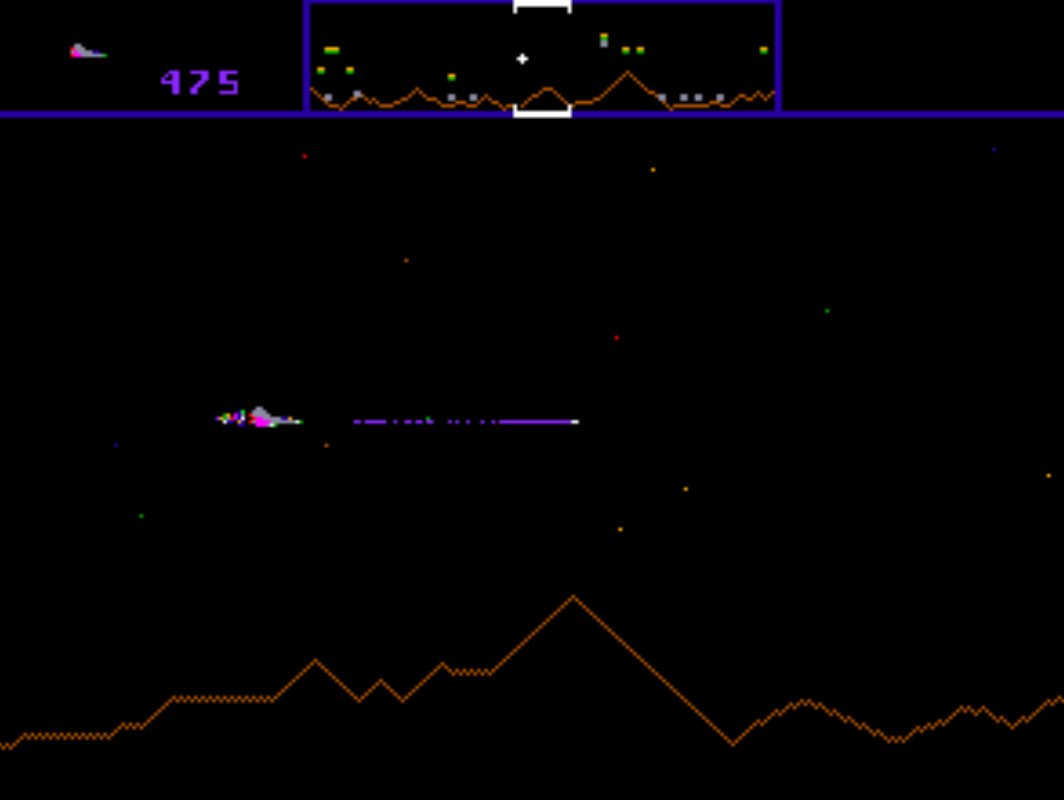
\includegraphics [scale=0.38]{defender} \newline

Defender is a 2D Side scrolling shooter, the controls were simple compared to today's style of games and control schemes, of course this didn't make the game any less difficult.

\clearpage

\subsubsection{R-Type (1987)}

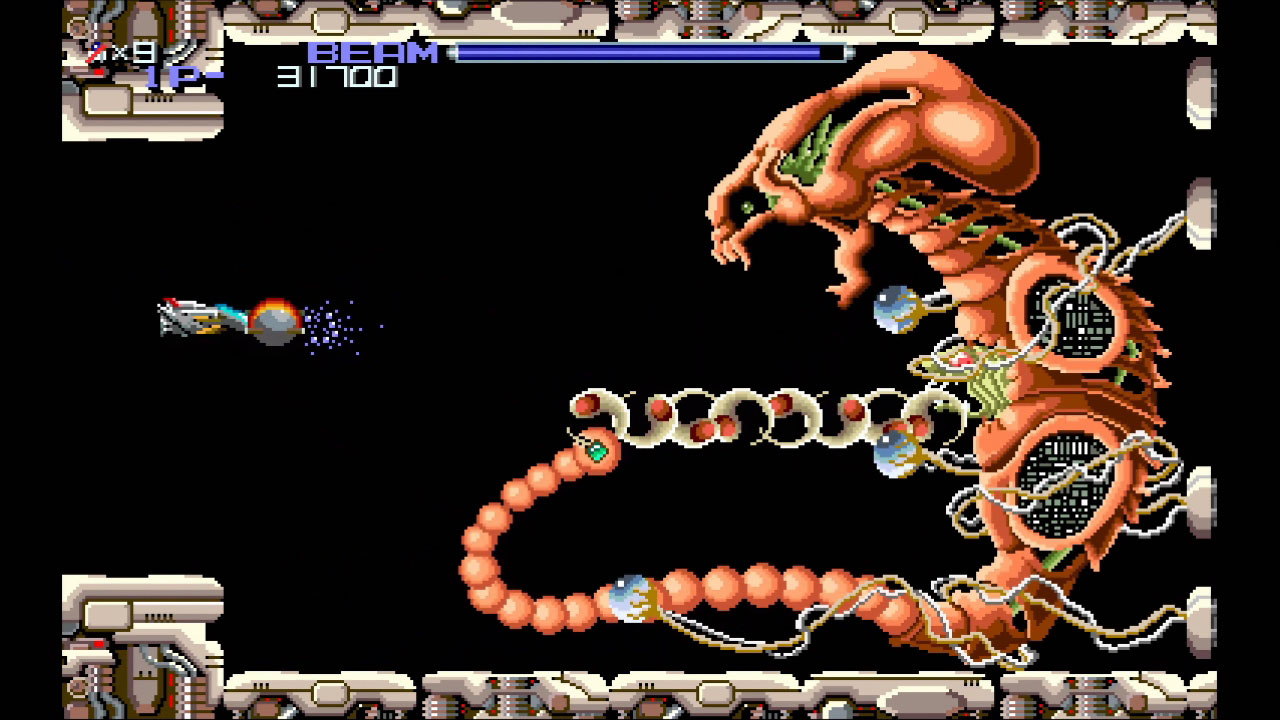
\includegraphics [scale=0.3]{rtype} \newline

R-Type is a side scrolling shoot-em-up arcade game produced by Irem in 1987. The player controls a space fighter named the R-9 with similar controls to defender, side scrolling shooter with the ability to move left, right, up and down.

R-Type was ported to various home platforms, and several of its versions including the arcade original have since been re-released on more contemporary consoles. Both the arcade game and the ports were well received by video game magazines. It has spawned a series of sequels by Irem and inspired several video games from other companies.

\clearpage		
			
\subsection{Platform}
\subsubsection{Super Mario(1980)}

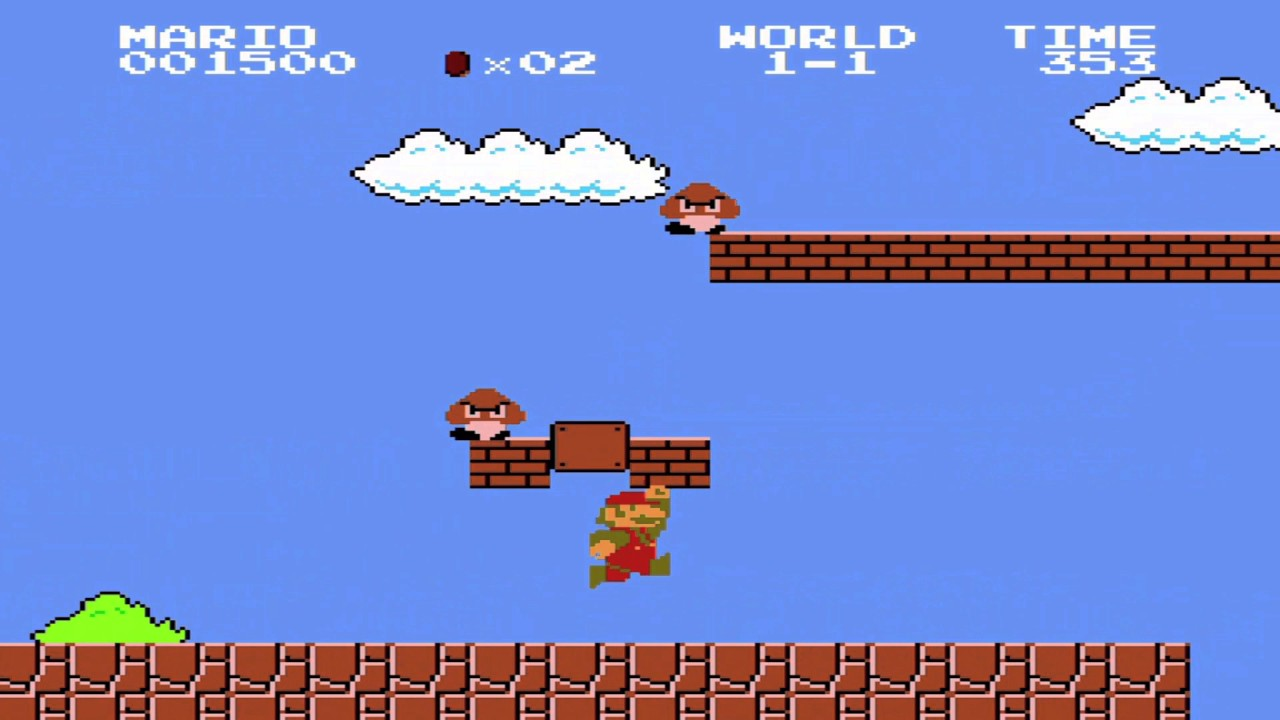
\includegraphics [scale=0.3]{mario} \newline

Super Mario is a series of fantasy platform games created by Nintendo featuring their mascot, Mario. Alternatively called the Super Mario Bros. series or simply the Mario series, it is the central series of the greater Mario franchise. At least one Super Mario game has been released for every major Nintendo video game console.

The Super Mario games follow Mario's adventures, typically in the fictional Mushroom Kingdom with Mario as the player character. He is often joined by his brother, Luigi, and occasionally by other members of the Mario cast. As in platform video games, the player runs and jumps across platforms and atop enemies in themed levels. The games have simple plots, typically with Mario rescuing the kidnapped Princess Peach from the primary antagonist, Bowser. The first title in the series, Super Mario Bros., released for the Nintendo Entertainment System (NES) in 1985, established gameplay concepts and elements prevalent in nearly every Super Mario game since. These include a multitude of power-ups and items that give Mario special magic powers such as fireball-throwing and size-changing into giant and miniature sizes.

The Super Mario series is part of the greater Mario franchise. This includes other video game genres as well as media such as film, television, printed media and merchandise. Over 310 million copies of games in the Super Mario series have been sold worldwide, as of September 2015, making it the best-selling video game series in history.

\clearpage

\subsubsection{Donkey Kong(1981)}
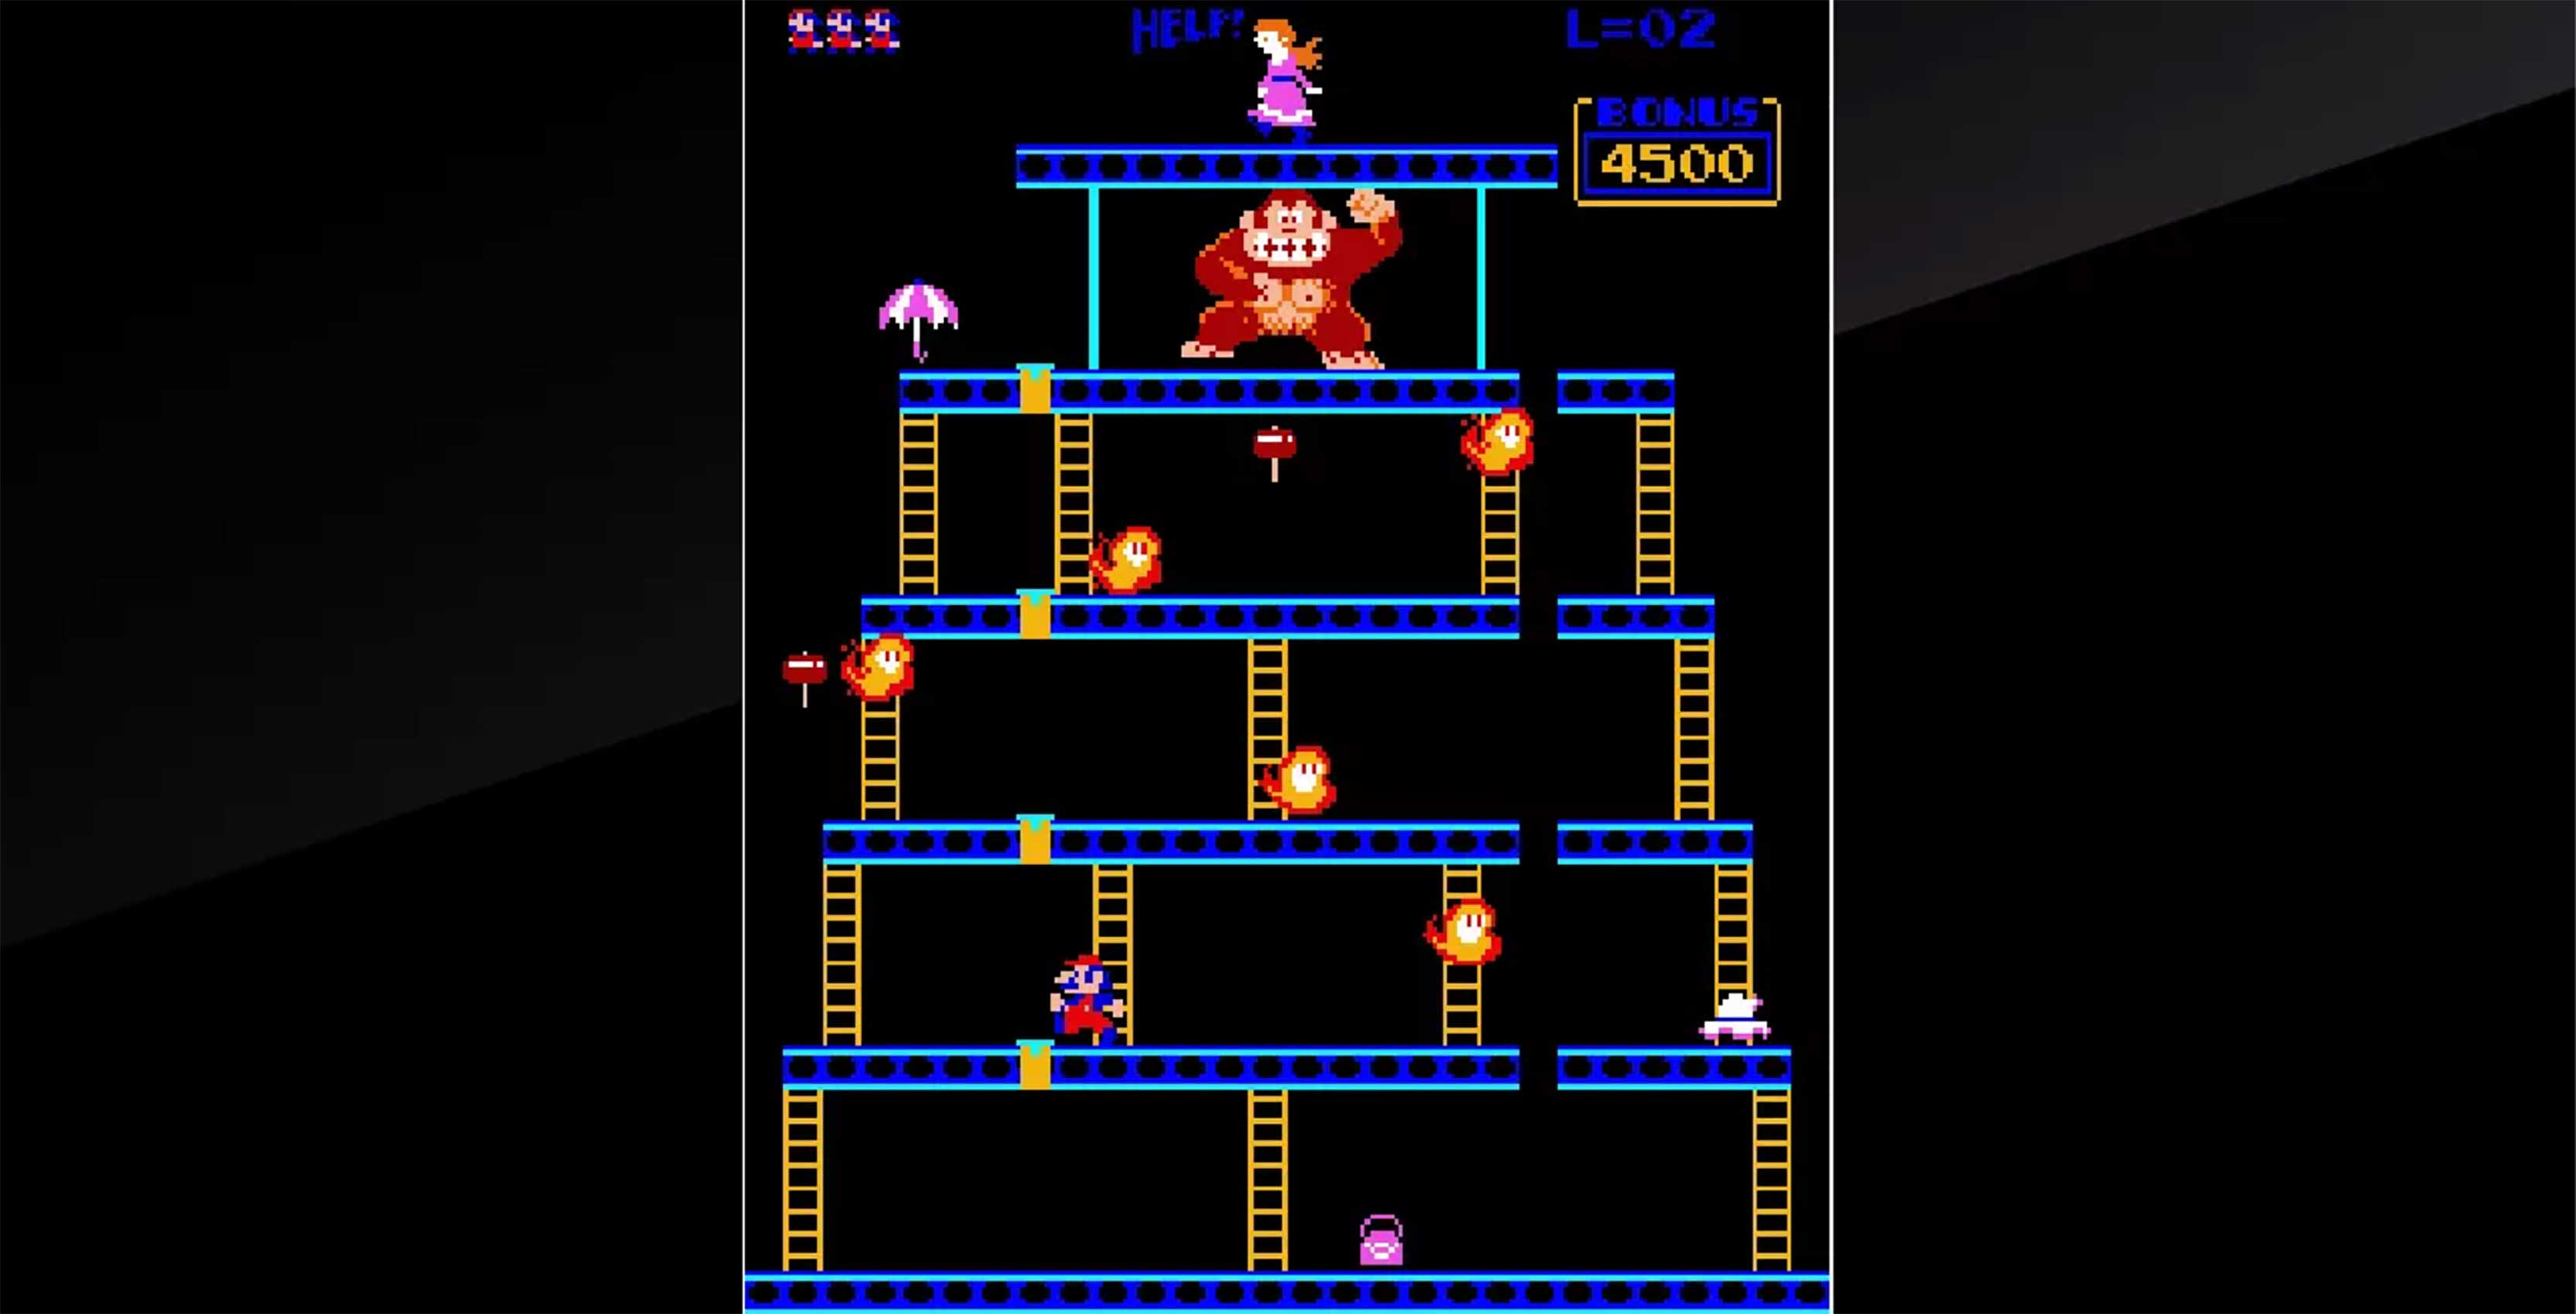
\includegraphics [scale=0.12]{donkeykong}
\clearpage
			
\subsection{Puzzle}
\subsection{Traditional Games}
	
\section{Design}
\subsection{Front End}
\subsection{In-Game Menus}
\subsection{Control Mechanisms}
\subsection{The Game}
\section{Game Mechanics}
\section{System Compatibility}
\section{Hardware Functions Used}
\section{Conclusion}
 
\end{document}